\chapter{Ideation}
\label{Ideation}
The very first ideation session was very far from the prototype that we ended up with. It started out as a classic brainstorm and ended up revolving around making a multi-purpose Near Field Communication (NFC) RFID device which would be able to toggle the correct signal on or off depending on where it should be used. This way it would be possible to have all your RFID purposes built in to one single device such as your credit card, Rejsekortet, your access card for the university etc. This would eliminate the need for fumbling around your wallet for the correct card of which there are many these days and perhaps even making it wearable eg. a ring on one's finger or embedded in one's jacket. However, the idea did not make it very far from the drawing board after a conversation with Markus Löchtefeld who had personal experience working with this technology. It was not deemed possible. We went back to idea creation and decided to make something fun. The idea of making something wearable carried over and eventually we settled on \textit{FingerDrums}, and idea that will make it possible to drum on any surface and then have a real drum sound play. 

The goal is now to develop an electrical instrument which will be able to simulate drum sounds. The instrument will have sensors attached to each finger, each having their own unique sound. When a finger drums on a surface the sound will play either via a loudspeaker or in a set of headphones. This allows for drumming on various surfaces, rigid or otherwise, as long as the appropriate resistance is met. The user is able to choose their preferred sound and assign it to the wanted finger. Some sort of interface is necessary for this action to be completed.

\section{Storyboard}
\label{storyboard}

In this section a storyboard, \autoref{fig:Storyboard}, featuring an ideal use case is shown, along with a short explanation of each pane.//

\begin{enumerate}
\item[\textbf{1}] The bus on the way to the university. 
\item[\textbf{2}] A person is listening to music through their headphones, and drumming along with their fingers.
\item[\textbf{3}] The sound of the drumming is a boring *Bum Bum*
\item[\textbf{4}] The person changes to a different finger but it produces the same boring *Bum Bum*
\item[\textbf{5}] The bus on the way home from the university. 
\item[\textbf{6}] A person is listening to music through their headphones, and drumming along with their fingers.
\item[\textbf{7}] The sound of the drumming is a deep bass-y *Bum Bum*
\item[\textbf{8}] The person changes to a different finger and produces a cool *Tish* -sound
\end{enumerate}


\begin{figure}[H]
\centering
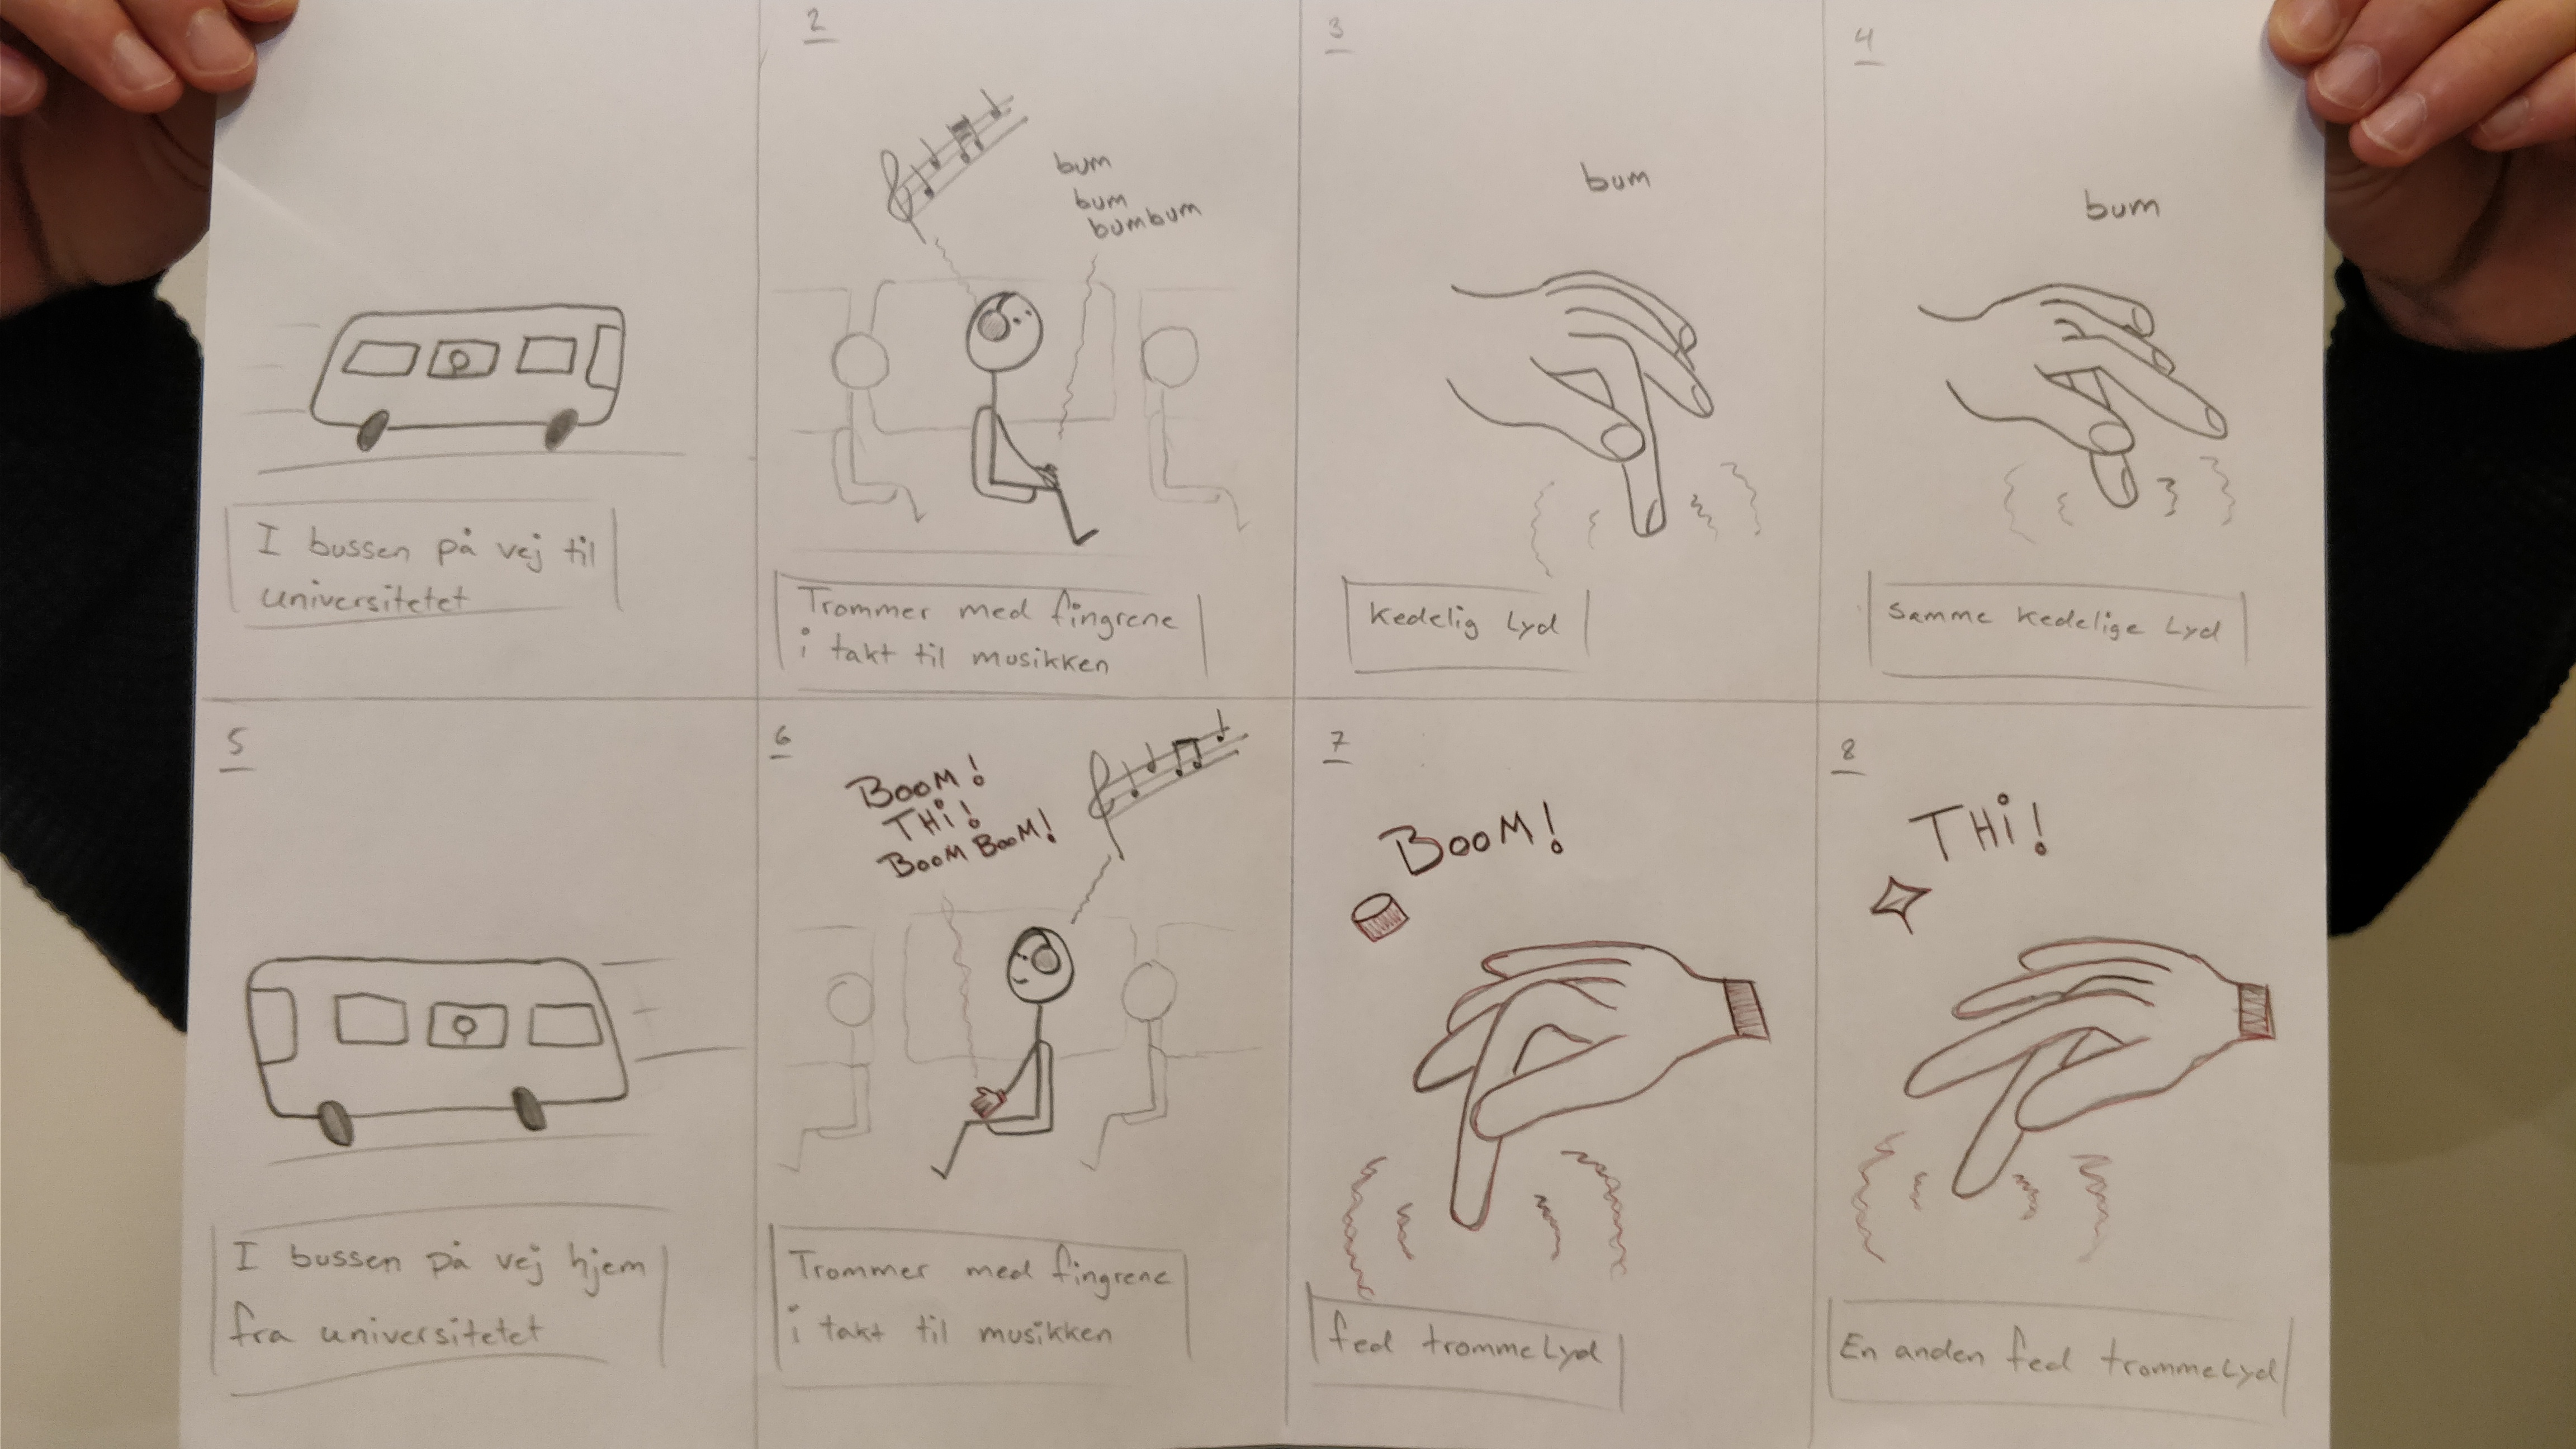
\includegraphics[width = \textwidth]{Figure/Billeder/IMG_20171114_121225.jpg}
\caption{Storyboard for a specific use case.}
\label{fig:Storyboard}
\end{figure}
\section{Verplank diagram}
\label{Verplank_diagram}
over the course of designing the fingerdrums a Verplan digram was created to help specify and explain the idea. 
\subsection{Idea}
Playing the drums on any surface using only your fingers as drumsticks.

\subsection{Metaphore}
Having a drum set in the palm of your hand that you can play at any time, in any place.

\subsection{Model}
Play the drums without being anywhere near an actual drum set.

\subsection{Display}
Small OLED display on the wrist which shows the type of drum set currently being used.

\subsection{Error}
Any touchscreens, for instance, your phone will not be usable when waring the glove. Drumming on any object will still produce a sound, which could be disruptive, depending on the object.

\subsection{Scenario}
You can play th drums on the bus on the way home from work without having to bring a actual drum set.

\subsection{Tasks}

\section{Sketching}
The first sketches of the \textit{FingerDrums} concept is seen in \autoref{fig:sketch_hand}. The idea was to attach a sensor at the fingertips to register the drumming and signal the drum sound. To the left on \autoref{fig:sketch_hand} a simple drum kit is also  sketched. Some questions arose relating to which finger should be playing what. Combined there are often more than seven drums or cymbals in total in a classic drum set-up which means that ideally both hands should be in use - not just the fingers, and perhaps it should be considered where else sensors could be attached in order to get a good experience of making a drum beat.\\
The sketch to the right on \autoref{fig:sketch_hand} challenges another possibility of interaction and show a small display attached to the user's wrist in order to see what drum sound is being played. That way the user would quickly be able to know and control which sound is playing and which sound they want to play

\begin{figure}[H]
\centering
\includegraphics[width = \textwidth]{Figure/sketch_hand}
\caption{The first sketch to the left illustrates the idea to attach FSR to the finger tips as a way of drumming on any surface while still sounding like a drumkit. The sketch to the right also represents the idea to attach FSR to the finger tips as a way of drumming on any surface while still sounding like a drumkit. A small OLED display has been added in this version as a way for the user to rapidly change the drum sounds if needed and is a form of feedback so that the user knows what sound profile is chosen.}
\label{fig:sketch_hand}
\end{figure}